\chapter{Core Foundations}

This block focuses on the fundamental structure of modern quantum computing:

\begin{center}
\textbf{How to represent, evolve, and optimize quantum systems using linear algebra and parametrized quantum circuits}
\end{center}

\vspace{0.5cm}

\section{QUANTUM COMPUTING (CORE)}

Quantum computing is a computational paradigm that leverages the principles of quantum mechanics 
to process information. Unlike classical computers, which use bits as the basic unit of 
information, quantum computers use quantum bits (qubits), enabling fundamentally 
new forms of computation.

\subsection{Qubit and Hilbert Space}

A qubit is not just a binary unit, but a vector in a complex Hilbert space, where its state 
is described by a superposition of basis states, enabling the rich structure of quantum 
computation.

A qubit represented by a vector in a 2-dimensional complex vector space:

\begin{equation}
|\psi\rangle = \alpha |0\rangle + \beta |1\rangle = 
\alpha
\begin{pmatrix}
1 \\
0
\end{pmatrix}
+
\beta
\begin{pmatrix}
0 \\
1
\end{pmatrix}
=
\begin{pmatrix}
\alpha \\
\beta
\end{pmatrix}
\end{equation}

with normalization condition:

\begin{equation}
|\alpha|^2 + |\beta|^2 = 1
\end{equation}

This naturally introduces:
\begin{itemize}
\item Linear algebra
\item Quantum probability
\end{itemize}

\subsection{Operators and Quantum Gates}

In quantum computing, operators and quantum gates are fundamentally the same 
mathematical objects viewed from different perspectives.

An operator is a linear transformation acting on vectors in a 
Hilbert space. In the context of a qubit. The evolution of a quantum state is given by:

\begin{equation}
|\psi'\rangle = \hat{U} |\psi\rangle
\end{equation}

where:
\begin{itemize}
\item $\hat{U}$ is a unitary operator
\item $\hat{U}^\dagger \hat{U} = I$
\end{itemize}

Examples of quantum gates:
\begin{itemize}
\item Pauli-X
\item Hadamard
\item CNOT
\end{itemize}

They operate on qubits and are analogous to classical logic gates, but they obey 
the principles of quantum mechanics.

\subsection{Single-Qubit Gates}

Single-qubit gates are the fundamental building blocks of quantum circuits. 
They act on a single qubit and correspond to unitary transformations in a 2-dimensional complex 
Hilbert space.

\subsubsection{Pauli-X Gate (NOT Gate)}

\begin{equation}
X =
\begin{bmatrix}
0 & 1 \\
1 & 0
\end{bmatrix}
\end{equation}

\textbf{What does it do?} It \textbf{flips the state of a qubit}, just like a classical NOT gate:

\begin{equation}
X|0\rangle = |1\rangle, \quad X|1\rangle = |0\rangle
\end{equation}

\textbf{Why is it called a NOT gate?}

In classical computing:
\[
\text{NOT}(0) = 1
\]
\[
\text{NOT}(1) = 0
\]

The Pauli-X gate performs exactly the same operation, but on a quantum bit (qubit).

\subsubsection{Action on a General State}

If a qubit is in a superposition:
\[
|\psi\rangle = \alpha |0\rangle + \beta |1\rangle
\]

Applying the Pauli-X gate:
\[
X|\psi\rangle = \alpha |1\rangle + \beta |0\rangle
\]

It swaps the amplitudes of $|0\rangle$ and $|1\rangle$.

\subsubsection{Geometric Interpretation (Bloch Sphere)}

\begin{itemize}
\item The Pauli-X gate corresponds to a rotation of $\pi$ radians around the $x$-axis.
\item It moves the qubit from the north pole to the south pole of the Bloch sphere.
\end{itemize}

\begin{figure}[h!]
\centering
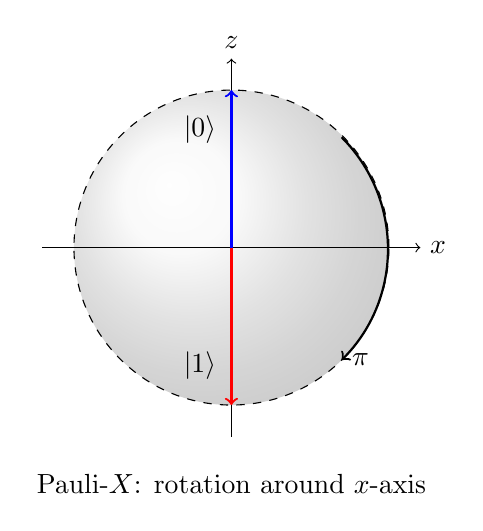
\begin{tikzpicture}[scale=2]

% Sphere
\shade[ball color=gray!20, opacity=0.3] (0,0) circle (1);

% Axes
\draw[->] (-1.2,0) -- (1.2,0) node[right] {$x$};
\draw[->] (0,-1.2) -- (0,1.2) node[above] {$z$};

% Equator
\draw[dashed] (0,0) circle (1);

% Poles
\node[above] at (-0.2,0.6) {$|0\rangle$};
\node[below] at (-0.2,-0.6) {$|1\rangle$};

% State vector before (north pole)
\draw[->, thick, blue] (0,0) -- (0,1);

% State vector after (south pole)
\draw[->, thick, red] (0,0) -- (0,-1);

% Rotation arrow (around x-axis)
\draw[->, thick] (0.7,0.7) arc[start angle=45,end angle=-45,radius=1]
node[below,right] {$\pi$};

% Label
\node at (0,-1.5) {Pauli-$X$: rotation around $x$-axis};

\end{tikzpicture}
\caption{Bloch sphere representation of the Pauli-$X$ gate}
\end{figure}

\noindent\rule{\textwidth}{1pt}

\subsubsection{Pauli-Y Gate}

\begin{equation}
Y =
\begin{bmatrix}
0 & -i \\
i & 0
\end{bmatrix}
\end{equation}

\begin{equation}
Y|0\rangle = i|1\rangle, \quad Y|1\rangle = -i|0\rangle
\end{equation}

\noindent\rule{\textwidth}{1pt}

\subsubsection{Pauli-Z Gate}

\begin{equation}
Z =
\begin{bmatrix}
1 & 0 \\
0 & -1
\end{bmatrix}
\end{equation}

\begin{equation}
Z|0\rangle = |0\rangle, \quad Z|1\rangle = -|1\rangle
\end{equation}

\noindent\rule{\textwidth}{1pt}

\subsubsection{Hadamard Gate}

The Hadamard gate creates a superposition of basis states.

\begin{equation}
H = \frac{1}{\sqrt{2}}
\begin{bmatrix}
1 & 1 \\
1 & -1
\end{bmatrix}
\end{equation}

Its action on the computational basis is given by:
\begin{equation}
H|0\rangle = \frac{|0\rangle + |1\rangle}{\sqrt{2}}, \quad
H|1\rangle = \frac{|0\rangle - |1\rangle}{\sqrt{2}}
\end{equation}

\begin{figure}[h!]
\centering

% ---------- FIRST FIGURE ----------
\begin{subfigure}[t]{0.48\textwidth}
\centering
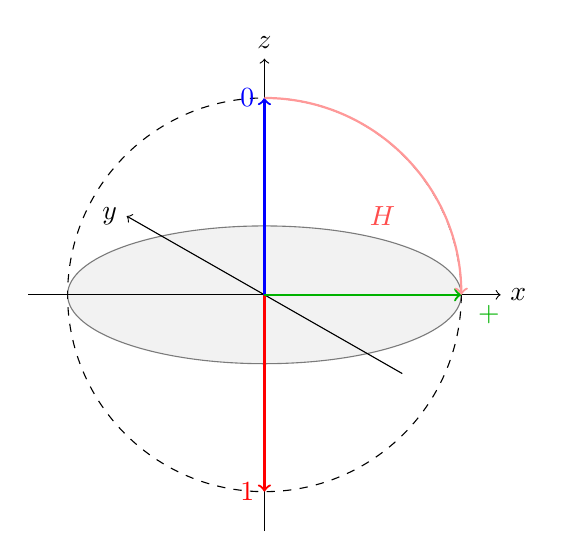
\begin{tikzpicture}[scale=2.5]

% Sphere
\draw[dashed] (0,0) circle (1);

% Equatorial plane
\draw[fill=gray!20, opacity=0.5] (0,0) ellipse (1 and 0.35);

% Axes
\draw[->] (0,-1.2) -- (0,1.2) node[above] {$z$};
\draw[->] (-1.2,0) -- (1.2,0) node[right] {$x$};
\draw[->] (0.7,-0.4) -- (-0.7,0.4) node[left] {$y$};

% |0> and |1>
\draw[->, thick, blue] (0,0) -- (0,1) node[left] {$\ket{0}$};
\draw[->, thick, red] (0,0) -- (0,-1) node[left] {$\ket{1}$};

% |+>
\draw[->, thick, green!70!black] (0,0) -- (1,0)
node[below] {$\hspace{0.7cm}\ket{+}$};

% Hadamard rotation arc
\draw[thick, red!40, ->]
(0,1) arc[start angle=90, end angle=0, radius=1];

\node[red!70] at (0.6,0.4) {$H$};

% Label
%\node at (0.7,1.1) {$H:\ \ket{0} \rightarrow \ket{+}$};

\end{tikzpicture}
\caption{$H:\ \ket{0} \rightarrow \ket{+}$}
\end{subfigure}
\hfill
% ---------- SECOND FIGURE ----------
\begin{subfigure}[t]{0.48\textwidth}
\centering
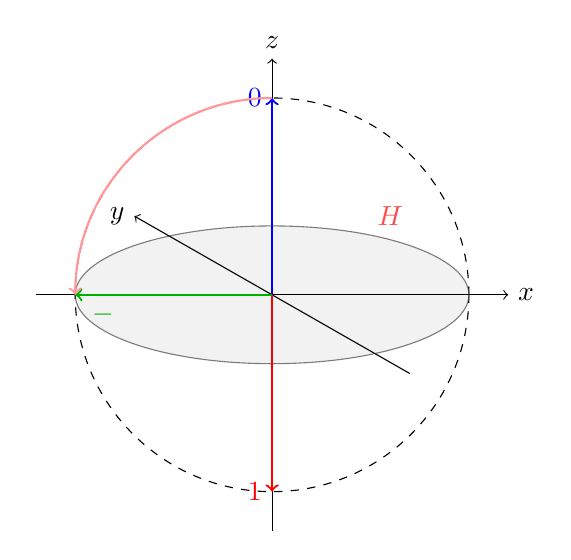
\begin{tikzpicture}[scale=2.5]

% Sphere
\draw[dashed] (0,0) circle (1);

% Equatorial plane
\draw[fill=gray!20, opacity=0.5] (0,0) ellipse (1 and 0.35);

% Axes
\draw[->] (0,-1.2) -- (0,1.2) node[above] {$z$};
\draw[->] (-1.2,0) -- (1.2,0) node[right] {$x$};
\draw[->] (0.7,-0.4) -- (-0.7,0.4) node[left] {$y$};

% |0> and |1>
\draw[->, thick, blue] (0,0) -- (0,1) node[left] {$\ket{0}$};
\draw[->, thick, red] (0,0) -- (0,-1) node[left] {$\ket{1}$};

% |+>
\draw[->, thick, green!70!black] (0,0) -- (-1,0)
node[right, below] {$\hspace{0.7cm}\ket{-}$};

% Hadamard rotation arc
\draw[thick, red!40, ->]
(0,1) arc[start angle=90, end angle=180, radius=1];

\node[red!70] at (0.6,0.4) {$H$};

% Label
%\node at (0.7,1.1) {$H:\ \ket{0} \rightarrow \ket{-}$};

\end{tikzpicture}
\caption{$H:\ \ket{0} \rightarrow \ket{-}$}
\end{subfigure}

\caption{Bloch sphere representation of the Hadamard transformation}
\end{figure}

\subsubsection{Phase Gates (S and T)}

\begin{equation}
S =
\begin{bmatrix}
1 & 0 \\
0 & i
\end{bmatrix}, \quad
T =
\begin{bmatrix}
1 & 0 \\
0 & e^{i\pi/4}
\end{bmatrix}
\end{equation}

\subsection{Multi-Qubit Gates}

\subsubsection{Controlled-NOT (CNOT) Gate}

The CNOT gate flips the target qubit if the control qubit is in state $|1\rangle$.

\begin{equation}
\text{CNOT} |10\rangle = |11\rangle
\end{equation}

Matrix representation:
\begin{equation}
\text{CNOT} =
\begin{bmatrix}
1 & 0 & 0 & 0 \\
0 & 1 & 0 & 0 \\
0 & 0 & 0 & 1 \\
0 & 0 & 1 & 0
\end{bmatrix}
\end{equation}

\subsubsection{SWAP Gate}

\begin{equation}
\text{SWAP} |ab\rangle = |ba\rangle
\end{equation}

\begin{equation}
\text{SWAP} =
\begin{bmatrix}
1 & 0 & 0 & 0 \\
0 & 0 & 1 & 0 \\
0 & 1 & 0 & 0 \\
0 & 0 & 0 & 1
\end{bmatrix}
\end{equation}

\subsubsection{Toffoli Gate (CCNOT)}

The Toffoli gate has two control qubits and one target qubit. The target qubit is flipped only if both control qubits are in state $|1\rangle$.

\subsection{Properties of Quantum Gates}

\begin{itemize}
\item All quantum gates are unitary (reversible transformations).
\item They preserve normalization of the quantum state.
\item They enable superposition and entanglement.
\end{itemize}

\subsection{Applications}

Quantum gates are essential for:
\begin{itemize}
\item Quantum algorithms (e.g., Shor's algorithm, Grover's algorithm)
\item Quantum cryptography
\item Quantum simulation
\end{itemize}

\subsection{Quantum Measurement}

Measurement probabilities:

\[
P(0) = |\alpha|^2, \quad P(1) = |\beta|^2
\]

After measurement, the state collapses to the observed eigenstate.

\vspace{0.5cm}

\section{PARAMETRIZED QUANTUM CIRCUITS (PQC)}

Parametrized Quantum Circuits (PQCs) are quantum circuits with adjustable parameters in their gates.
These parameters are typically optimized using classical algorithms in a hybrid approach.
PQCs are widely used in variational quantum algorithms like VQE and QAOA.
They are suitable for near-term quantum devices with limited coherence.
By tuning parameters, PQCs aim to minimize a cost function and solve complex problems.


These are the foundation of:
\begin{itemize}
\item Variational algorithms (VQE, QAOA)
\item Quantum machine learning
\end{itemize}

\subsection*{General Form}

\[
|\psi(\theta)\rangle = U(\theta) |0\rangle
\]

where $\theta$ represents tunable parameters.

Typical parametrized gates:

\[
R_x(\theta), \quad R_y(\theta), \quad R_z(\theta)
\]

\subsection*{Core Idea}

Optimization problem:

\[
\min_{\theta} \langle \psi(\theta) | H | \psi(\theta) \rangle
\]

This is known as \textbf{variational optimization}.

\vspace{0.5cm}

\section{VARIATIONAL QUANTUM EIGENSOLVER (VQE)}

The Variational Quantum Eigensolver (VQE) is a hybrid quantum-classical algorithm used to estimate the ground state energy of a quantum system.
It combines a parametrized quantum circuit with a classical optimizer to minimize the energy expectation value.
The quantum computer prepares trial states, while the classical computer updates the parameters iteratively.
VQE is especially useful for problems in quantum chemistry and materials science.
It is well-suited for noisy intermediate-scale quantum (NISQ) devices.


\subsection*{Objective}

To find the ground state energy of a Hamiltonian.

\subsection*{Eigenvalue Problem}

\[
H |\psi\rangle = E |\psi\rangle
\]

\subsection*{Strategy}

\begin{enumerate}
\item Choose a parametrized ansatz
\item Compute expectation value
\item Minimize using classical optimization
\end{enumerate}

\[
E(\theta) = \langle \psi(\theta) | H | \psi(\theta) \rangle
\]

\subsection*{Physical Interpretation}

Approximation of the lowest eigenvalue of $H$.

\vspace{0.5cm}

\section{QUANTUM APPROXIMATE OPTIMIZATION ALGORITHM (QAOA)}

The Quantum Approximate Optimization Algorithm (QAOA) is a hybrid quantum-classical algorithm designed to solve combinatorial optimization problems.
It uses a parametrized quantum circuit with alternating operators to explore the solution space.
A classical optimizer adjusts the parameters to maximize or minimize a given cost function.
QAOA is particularly effective for problems like Max-Cut and other graph-based optimizations.
It is well-suited for implementation on noisy intermediate-scale quantum (NISQ) devices.

\subsection*{Applications}

\begin{itemize}
\item Combinatorial optimization (e.g., Max-Cut)
\end{itemize}

\subsection{State Construction}

\[
|\gamma, \beta\rangle = e^{-i\beta H_M} e^{-i\gamma H_C} |+\rangle
\]

where:
\begin{itemize}
\item $H_C$: cost Hamiltonian
\item $H_M$: mixing Hamiltonian
\end{itemize}

\subsection*{Key Idea}

Alternate between:
\begin{itemize}
\item Cost evolution
\item Mixing evolution
\end{itemize}

This resembles:
\begin{itemize}
\item Trotterization
\item Controlled quantum dynamics
\end{itemize}

\vspace{0.5cm}

\section{SIMULATION OF QUANTUM SYSTEMS}

Simulation of Quantum Systems involves using computational methods to model the behavior of quantum mechanical systems.
Quantum computers can efficiently simulate systems that are intractable for classical computers.
This is particularly important in quantum chemistry, materials science, and condensed matter physics.
Techniques such as PQCs and algorithms like VQE are often employed for these simulations.
Such simulations enable the study of molecular structures, reaction dynamics, and physical properties.

\subsection*{Time Evolution}

\[
|\psi(t)\rangle = e^{-iHt} |\psi(0)\rangle
\]

\subsection*{Methods}

\begin{itemize}
\item Exact matrix exponentiation
\item Trotter-Suzuki decomposition
\item Variational simulation
\end{itemize}

\subsection*{Connection to Physics}

Time evolution follows the Schrödinger equation:

\[
i\hbar \frac{d}{dt} |\psi\rangle = H |\psi\rangle
\]

\vspace{0.5cm}

\section*{MATHEMATICAL FOUNDATION}

\subsection*{6.1 Linear Algebra}

\subsubsection*{Complex Vector Spaces}

\begin{itemize}
\item Orthonormal basis
\item Inner product:
\[
\langle \psi | \phi \rangle
\]
\end{itemize}

\subsubsection*{Linear Operators}

Hermitian operators:

\[
A = A^\dagger
\]

These represent physical observables.

\subsubsection*{Eigenvalues and Eigenvectors}

\[
A |v\rangle = \lambda |v\rangle
\]

Applications:
\begin{itemize}
\item Energy levels
\item Measurement outcomes
\end{itemize}

\subsubsection*{Spectral Decomposition}

\[
A = \sum_i \lambda_i |v_i\rangle \langle v_i|
\]

\vspace{0.5cm}

\subsection*{6.2 Quantum Mechanics}

\subsubsection*{Postulates}

\begin{enumerate}
\item State: vector in Hilbert space
\item Observables: Hermitian operators
\item Measurement: eigenvalues
\item Evolution: unitary
\item Composite systems: tensor product
\end{enumerate}

\subsubsection*{Tensor Product}

\[
|00\rangle, |01\rangle, |10\rangle, |11\rangle
\]

Foundation for:
\begin{itemize}
\item Entanglement
\item Multi-qubit systems
\end{itemize}

\subsubsection*{Measurement Operators}

\[
P_i = |v_i\rangle \langle v_i|
\]

\vspace{0.5cm}

\section*{FINAL CONNECTION}

All concepts reduce to four pillars:

\begin{enumerate}
\item \textbf{Representation:} state vectors
\item \textbf{Transformation:} unitary operators
\item \textbf{Measurement:} Hermitian operators
\item \textbf{Optimization:} parameter tuning
\end{enumerate}

\vspace{0.5cm}

\section*{STUDY ROADMAP}

\subsection*{Phase 1 --- Mathematics}
\begin{itemize}
\item Complex vector spaces
\item Inner product
\item Eigenvalues and eigenvectors
\item Hermitian operators
\end{itemize}

\subsection*{Phase 2 --- Quantum Mechanics}
\begin{itemize}
\item Postulates
\item Measurement theory
\item Time evolution
\item Composite systems
\end{itemize}

\subsection*{Phase 3 --- Quantum Computing}
\begin{itemize}
\item Qubits
\item Quantum gates
\item Circuits
\end{itemize}

\subsection*{Phase 4 --- Variational Methods}
\begin{itemize}
\item Parametrized circuits
\item VQE
\item QAOA
\end{itemize}

\subsection*{Phase 5 --- Implementation}
\begin{itemize}
\item Python-based quantum frameworks
\item Simulation and experimentation
\end{itemize}